\documentclass[a4paper, 12pt]{article}
\usepackage[utf8]{inputenc}
\usepackage{geometry}
\usepackage{polski}
\usepackage{graphicx}
\usepackage{float}
\usepackage{etoolbox,refcount}
\usepackage{multicol}
\usepackage{tabularx}

\newgeometry{left=2cm, right=2cm, bottom=2cm, top=1.5cm}

\begin{document}
	\begin{figure}[H]
		\centering
		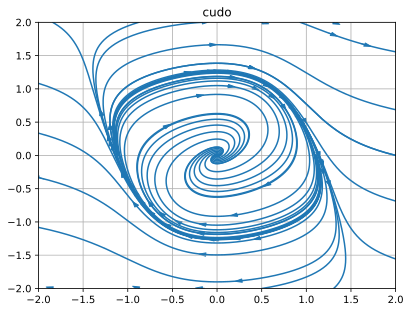
\includegraphics[width = \textwidth]{./img/cudo.png}
	\end{figure}
	\section{Cel ćwiczenia}
		Celem ćwiczenia jest zapoznanie się z przykładowym oprogramowaniem pozwalającym na realizację sterowania cyfrowego w oparciu o komputer klasy PC oraz zapoznanie się z przykładem interfejsu procesowego dla komputera klasy PC.
	\section{Budowa stanowiska}
		Stanowisko składa się z modelowegu układu śledzenia pozycji słońca pozwalającego na niezależny obrót baterii słonecznych wokół osi pionowej (azymut) i poziomej (elewacja). Układ posiada czujnik oświetlenia pozwalający na zmierzenie poziomu oświetlenia padającego z danego kierunku oraz czujniki krańcowe, które informują o osiągnięciu przez ogniwo maksymalnego odchylenia. Czujniki krańcowe współdziałają z wyłącznikami ruchu zabezpieczając układ przed uszkodzeniem.
		\begin{figure}[H]
			\centering
			\includegraphics[width = 0.6\textwidth]{./img/bad_motors.png}
			\includegraphics[width = 0.39\textwidth]{./img/ogniwa.png}
			\caption{Stanowisko}
		\end{figure}
		\noindent
		Silniki używane do poruszania ogniwem zasilane są prądem stałym o napięciu 12$\,$V. Sterowanie nimi odbywa się przy pomocy modułu przekaźnikowego ADAM4060. Napięciowe sygnały analogowe są podawane na wejścia modułu ADAM4018, a dyskretne sygnały z wyłączników krańcowych odbiera moduł ADAM4050. Wszystkie moguły są połączone magistralą RS486, a następnie za pośrednictwem modemu radiowego z komputerem.
	\section{Wprowadzenie}
		Ze względu na ograniczenia narzucone przez moduł ADAM4060 -- posiada dwa wyjścia\linebreak typu A oraz dwa wyjścia typu C -- sterowanie musi być zrealizowane jak jest pokazane na schemacie. Nie jest to jednak optymalnie zbudowany układ, gdyż nie pozwala on na wykonanie ruchu po jednej z przekątnych. Jednak taki układ silników jest wystarczający dla paneli słonecznych ze względu na tempo w jakim mają nadążać za słońcem. Sygnalizacja na wyjściach w module ADAM4060 w logice odwrotnej:
		\begin{center}
			\begin{tabularx}{\textwidth}{@{\extracolsep{\fill}} |l|c|c|c|c|}
				\hline
				Ruch$\backslash$Przekaźnik & R1(bit 0) & R2(bit 1)& R3(bit 2)& R4(bit 3) \\ \hline
				Do góry    & 0 & 1 & 0 & 1\\ \hline 
				Na dół 	   & 0 & 1 & 1 & 0\\ \hline
				W lewo     & 1 & 0 & 1 & 0\\ \hline
				W prawo    & 1 & 0 & 0 & 1\\ \hline
				Dół--lewo  & 1 & 1 & 1 & 0\\ \hline
				Dół--prawo & 1 & 1 & 0 & 1\\ \hline
				Góra--lewo & \multicolumn{4}{c|}{Niemożliwe} \\ \hline
				Dół--prawo & \multicolumn{4}{c|}{Niemożliwe} \\ \hline
			\end{tabularx}
		\end{center}
		Ponieważ ruch panelu jest ograniczony przez czujniki krańcowe, wyłączniki ruchu i inne rozwiązania sprzętowe nie jest konieczna implementacja ograniczeń ruchowych w strategii.
	\section{Przeprowadzenie ćwiczenia}
		Poniższy schemat przedstawia zaimplementowaną przez nas strategię. Wykorzystaliśmy w niej bloczki alternatywy logicznej, tagi, wyjścia dyskretne sterujące pracą silników, wejścia cyfrowe pokazujące stan czujników krańcowych, dwa wejścia analogowe od czujników azymutu oraz elewacji oraz cztery wejścia analogowe połączone z czujnikami mierzącymi poziom oświetlenia.
		\begin{figure}[H]
			\centering
			\includegraphics[width = 0.9\textwidth]{./img/strategy.png}
			\caption{Strategia}
		\end{figure}
		\noindent
		Wyjścia cyfrowe są połączone numeracją tak samo jak przełączniki w tabelce (DOx jest połączony z Rx) Poszczególne tagi są połączone z przyciskami Display'a: 
		\begin{itemize}
			\item[--] BBTN1 -- left
			\item[--] BBTN2 -- right
			\item[--] BBTN3 -- down
			\item[--] BBTN4 -- up
		\end{itemize}
		Przypadki niemożliwe takie jak próba poruszania się w przeciwnych kierunkach lub po niemożliwej osi oraz funkcjonalność klawisza ,,stop'' została przez nas zrealizowana poprzez wybijanie przycisków odpowiedzialnych za sterowanie. Sterowanie jest możliwe przy pomocy klawiszy z klawiatury.
		\begin{figure}[H]
			\centering
			\includegraphics[width = 0.9\textwidth]{./img/display.png}
			\caption{Display}
		\end{figure}
		\noindent
		Wyświetlacz ,,horizontal'' wyświetla azymut, a ,,vertical'' elewację. Kontrolki odpowiadające za wskazywanie stanu czujników krańcowych zmieniają kolor w chwili osiągnięcia maksymalnego kąta obrotu przez silniki. Wyświetlacze znajdujące się na przedłużeniach klawiszy sterujących wskazują odpowiednie poziomy naświetlenia.
	\section{Wnioski i obserwacje}
		Ćwiczenie zostało zakończone powodzeniem. Udało się zrealizować układ sterowania ogniwami słonecznymi, reagujący na wciśnięcie klawiszy z wykluczeniem sytuacji niemożliwych wynikających z ograniczeń fizycznych obiektu.
		\newline
		\newline
		Dużym ograniczeniem tego układu sterowania jest brak możliwości równoczesnego poruszania się ogniwa do góry i w lewo oraz w dół i w prawo. Istnieje jednak możliwość ominięcia tego dzięki zastosowaniu czterech wyjść przełącznikowych. 
		\begin{figure}[H]
			\centering
			\includegraphics[width = 0.8\textwidth]{./img/good_motors.png}
		\end{figure}
		\noindent Dzięki takiemu rozwiązaniu obydwa silniki mogą kręcić się niezależnie w obydwie strony, co eliminuje problem niemożności ruchu po jednej z przekątnych.
		\newline
		\newline 
		Zapoznaliśmy się z działaniem czujników krańcowych oraz ich budową. Wraz z wyłącznikami tworzą dobry system zabezpieczający układ przed uszkodzeniami wynikającymi ze zbyt dużych kątów wychylenia.
		\newline
		\newline 
		Dowiedzieliśmy się o kolejnych funkcjonalnościach oprogramowania VisiDAQ/GeniDAQ oraz wiemy jak je wykorzystać do zrealizowania sterowania. Zamiast komplikować strategię w naszym programie postanowiliśmy skorzystać z funkcji wybijania klawiszy oferowanej przez ustawienie typu klawisza na ,,Radio Button''.
\end{document}
